\section{Técnicas de Deep Learning y métodos de evaluación}

\subsection{Explicar las técnicas de DL que se van a utilizar en el proyecto}

% (Esto sería parte teórica)

{\color{red} \textbf{!!! TODO}}

\begin{itemize}
	\item mencionar transfer learning
	\item redes convolucionales
\end{itemize}

Para el entrenamiento se ha utilizado la técnica \textit{hold-out}, que consiste en dividir el conjunto de datos en dos subconjuntos: uno que será utilizado para la fase de entrenamiento y el otro que será utilizado para evaluar el modelo entrenado. Dada la escasez de imágenes no se ha utilizado un conjunto de validación durante el entrenamiento.

\subsection{Explicar los métodos de evaluación que se van a utilizar en el proyecto}

En los problemas de detección de objetos en imágenes se tienen por un lado una serie de regiones definidas en cada una de las imágenes que se corresponden con los objetos que se tienen que detectar. Y por otro lado se tiene un listado de regiones con los las predicciones de objetos que se han realizado.

La métrica que se ha utilizado para evaluar el modelo obtenido es la \textit{AP} (Average Precision), que es la métrica que se utiliza para evaluar modelos de detección de objetos.

Antes de explicar en qué consiste la métrica \textit{AP} hay que explicar una serie de conceptos en los cuales está basada: IoU (intersección sobre la unión), precisión (precision) y sensibilidad (recall).

El concepto de \textit{IoU} mide cuánto se solapan dos regiones: la predicha y la que debería ser detectada. Se calcula dividiendo la región obtenida mediante la intersección de la región predicha y la región a detectar entre la región obtenida mediante la unión de ambas regiones.

%2*\includegraphics{image1} + 3*\includegraphics{image2} = \includegraphics{image3}
\begin{equation}
	AP = \frac{interseci\acute{o}n}{uni\acute{o}n} = \frac{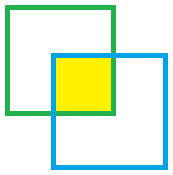
\includegraphics[width=0.2\linewidth]{images/ap_intersection.png}}{
\includegraphics[width=0.2\linewidth]{images/ap_union.png}}
	\nonumber
\end{equation}

La \textit{precisión} (precision) mide la capacidad del modelo para detectar únicamente los objetos relevantes. Se calcula como el porcentaje de predicciones positivas acertadas frente a todas las predicciones positivas predichas:

\begin{equation}
	precisi\acute{o}n = \frac{TP}{TP + FP} = \frac{TP}{todas\ las\ predicciones\ positivas}
	\nonumber
\end{equation}

La \textit{sensibilidad} (recall)  mide la capacidad del modelo para detectar todos los objetos relevantes. Se calcula como el porcentaje de predicciones positivas acertadas frente a todas las existentes:

\begin{equation}
	sensibilidad = \frac{TP}{TP + FN} = \frac{TP}{todas\ las\ regiones\ a\ detectar}
	\nonumber
\end{equation}

Tanto en el cálculo de la \textit{precisión} como en el cálculo de la \textit{sensibilidad}, para determinar si una predicción es positiva, se utiliza el \textit{IoU}. Se define un umbral para el \textit{IoU} (normalmente suele ser 0.5) y si se supera dicho umbral, la predicción es considerada una predicción positiva.

La métrica \textit{AP} se calcula como el área debajo de la curva \textit{precisión-sensibilidad} (precision-recall). En el eje de las abscisas se representa la \textit{sensibilidad} (recall) y en el eje de las ordenadas se representa la \textit{precisión} (precision).

A continuación se va a mostrar un ejemplo práctico de cómo se calcula la \textit{AP}. Para este ejemplo se dispone de una serie de imágenes con un total de 4 socavones a detectar. En la figura \ref{fig:apprecisionrecalltable} se puede ver el cálculo de la \textit{precisión} y de la \textit{sensibilidad} para las predicciones obtenidas. La columna \textit{Positivo} indica si la predicción es positiva, es decir, si el valor de \textit{IoU} supera el umbral definido, que en este caso es 0.5. Las columnas \textit{TP} y \textit{FP} muestran el acumulado de sus respectivos valores.

\begin{figure}[H]
	\centering
	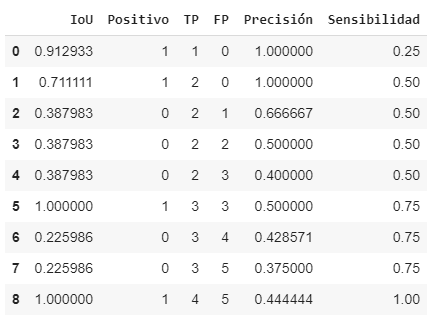
\includegraphics[width=0.6\linewidth]{images/ap_precision_recall_table.png}
	\caption{Cálculo de la precisión y sensibilidad para las predicciones}
	\label{fig:apprecisionrecalltable}
\end{figure}

Una vez se tienen calculados los valores de \textit{precisión} y de \textit{sensibilidad} se calcula la curva \textit{precisión-sensibilidad} como se puede ver en la figura \ref{fig:apprecisionrecallcurve}. Para realizar el cálculo del área debajo de la curva se realiza un suavizado de la misma. Este suavizado consiste en establecer como valor de \textit{precisión} para un determinado valor de \textit{sensibilidad}, el valor de \textit{precisión} más alto que se encuentre a su derecha. Por ejemplo, para la \textit{sensibilidad} 0.6 se establece como valor de \textit{precisión} el valor más alto a su derecha, que en este caso es 0.5. En color naranja se puede ver la curva suavizada.

\begin{figure}[H]
	\centering
	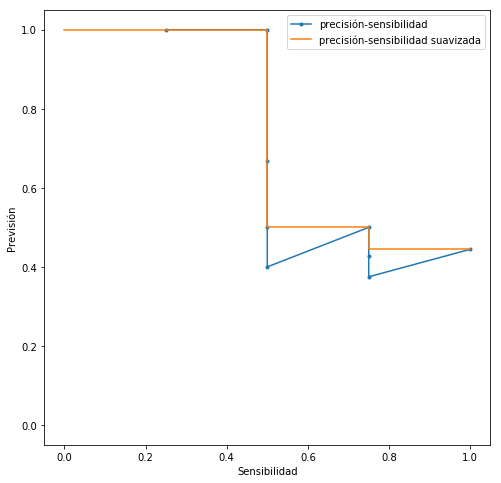
\includegraphics[width=0.7\linewidth]{images/ap_precision_recall_curve.png}
	\caption{Curva precisión-sensibilidad}
	\label{fig:apprecisionrecallcurve}
\end{figure}

Por lo que finalmente, para este ejemplo, el cálculo del \textit{AP} sería:

\begin{equation}
	AP = (0.5 - 0) \cdot 1 + (0.75 - 0.5) \cdot 0.5 + (1 - 0.75) \cdot 0.44 = 0.5 + 0.125 + 0.11 = \textbf{0.735}
	\nonumber
\end{equation}